\label{ch:prog-doc}
\section{Übersicht}
Das im Zuge dieser Diplomarbeit entwickelte Software-Projekt basiert auf einer den von Microsoft bereitgestellten Xamarin.Forms-Vorlagen, welche als Teil von Visual Studio bereitgestellt werden.
Es gibt mehrere Auswahlmöglichkeiten, wobei alle Vorlagen bis auf \enquote{Blank} Beispielcode beinhalten.
Da der Beispielcode der anderen Vorlagen für dieses Projekt nicht relevant ist und ohnehin gelöscht werden müsste, wird die \enquote{Blank}-Vorlage verwendet.
Diese Vorlage beinhaltet nur eine Haupt-Oberflächenseite ohne jeglichen Beispielcode.

Der immer wieder vorkommende Name PiBell ist eine freigeistliche Erfindung. PiBell ist der Projektname, der sich aus \acl{rpi} und \enquote{Bell}, dem englischen Wort für Klingel oder Glocke, zusammensetzt.

Visual Studio organisiert alle Programmteile in einer sogenannten Solution, welche diesen Projektnamen trägt. In diesem Fall beinhaltet die Solution \enquote{PiBell} drei Programmteile oder \enquote{Projects}.
Dieser Aufbau wird in Abbildung \ref{fig:solution} dargestellt.

\paragraph{PiBell} ist das portable Projekt, auch \ac{dotnet}-Standard-Projekt genannt.
Dieses beinhaltet den ganzen plattformunabhängigen Code, sowie die Definition der \ac{ui}-Oberfläche mittels \ac{xaml}-Dateien.
In diesem Projekt befindet sich der größte entwickelte Code-Anteil, da die meisten Funktionen, wie das Abspielen von Videos mit Hilfe der LibVLC-Bindings, plattformunabhängig funktionieren und deswegen geteilt werden können.

\paragraph{PiBell.Android} beinhaltet allen Code, der plattformspezifisch für Android geschrieben wurde.
Unter anderem ist hier die Android-Implementation des Mikrofon-Auf\-nahme-Services, sowie das Berechtigungs-Management enthalten.
Die Mikrofon-Aufnahme erfolgt auf einer sehr hardwarenahen Ebene, was die Plattform-Abhängigkeit erklärt.

\paragraph{PiBell.iOS} beinhaltet wie PiBell.Android den plattformspezifischen Code für die iOS-Platt\-form. Aufgrund mangelnder Entwicklungswerkzeuge wird dieser Teil nur am Rande gestreift.\par

\begin{figure}
\centering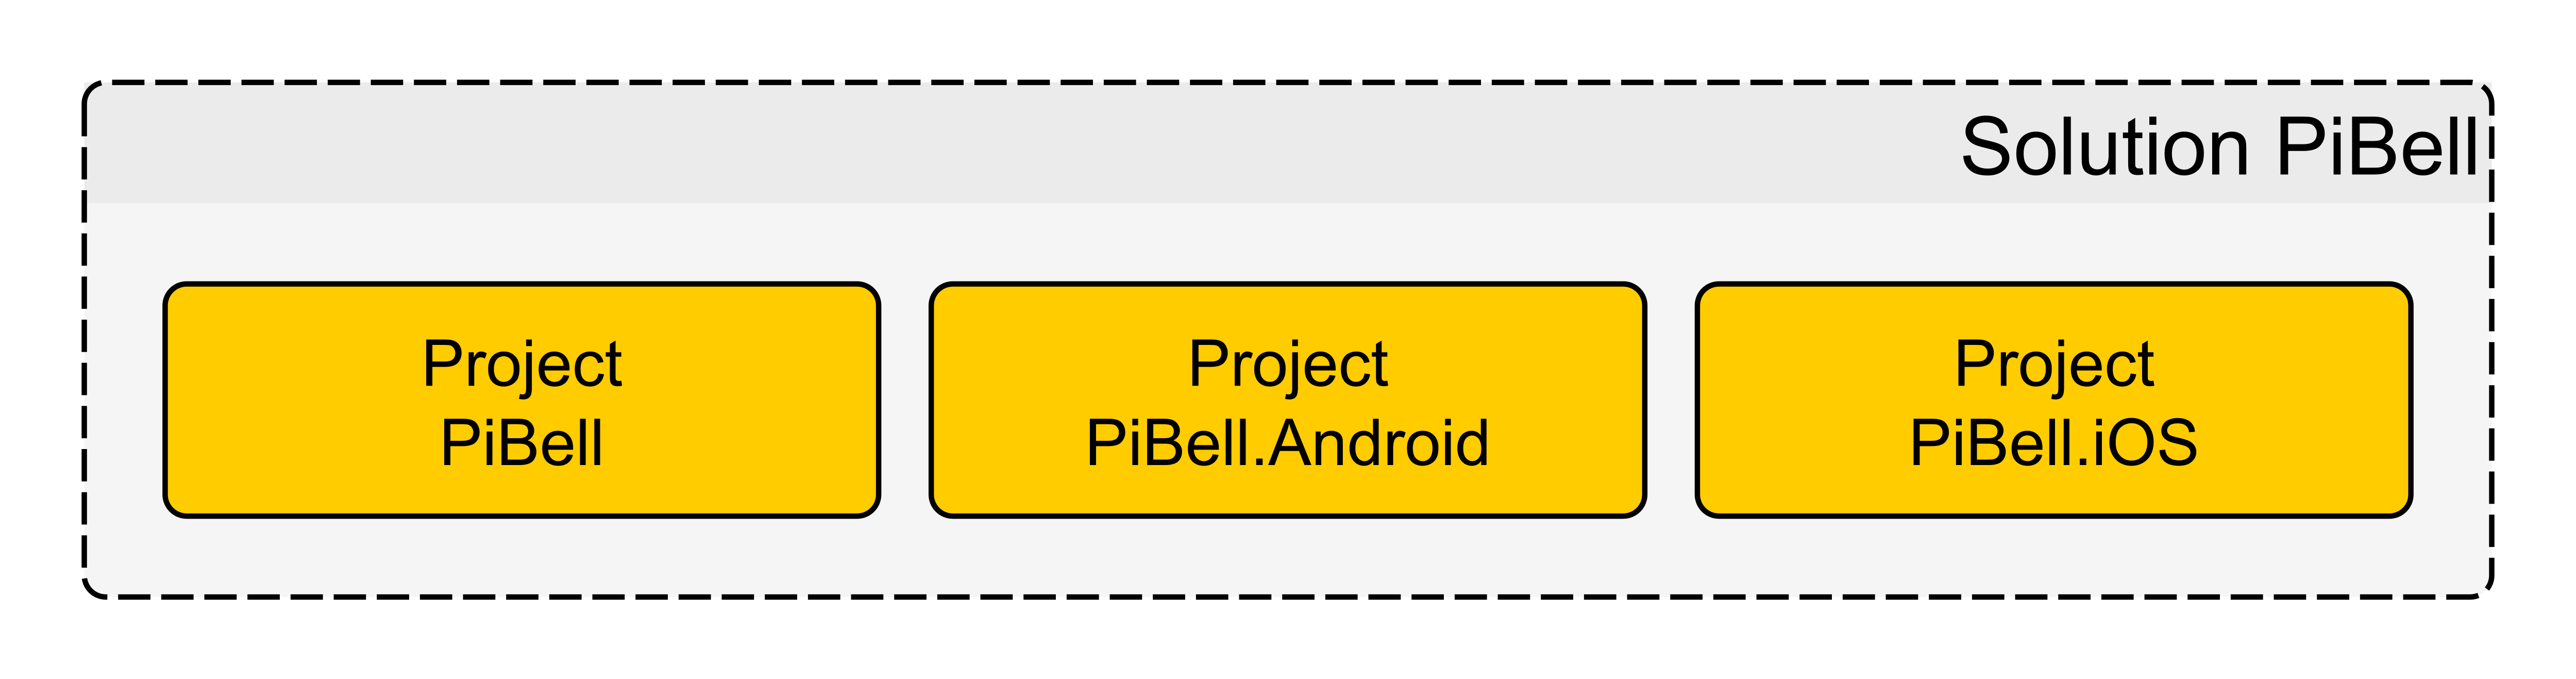
\includegraphics[width=0.9\linewidth]{images/xamarin/struktur.png}
\caption{Aufbau der Solution}
\label{fig:solution}
\end{figure}

%besteht aus drei teilen
%- portable project/.net standard project
%   plattformunabhängiger teil, oberfläche, ...
%- Android project
    %android-spezifischer teil, berechtigungen, ...
%- iOS project
    %iOS-spezifischer Teil, ...
%project-name PiBell -> erfindung, leitet sich aus raspberry und Türglocke ab
%
\section{Portable Project}
Im folgenden Teil werden die wesentlichen Teile des portablen Projektes PiBell beschrieben.
In den einzelnen Programmteilen gibt es immer wiederkehrende Abläufe, wie Initialisierung, die nur einmal beschrieben werden.
Die von Microsoft vorgefertigten Teile werden nicht behandelt.
Der Fokus liegt damit auf den selbst erstellten Programmteilen.
Die Programmteile werden generell in derselben Reihenfolge behandelt, wie sie vom Programm aufgerufen werden.\par

Textsegmente mit vorgestellter Zeilennummer sind direkt vom Programm eingefügt worden.
Der beschreibende Text bezieht sich auf den Programmteil mit Hilfe der Zeilennummern.

\subsection{App.xaml.cs}
\label{ssec:app-xaml-cs}
Im diesem Programmteil wird die Applikation grundlegend initialisiert.
Die Initialisierung beinhaltet unter anderem das Laden aller benötigten Programm-Bibliotheken und NuGet-Pakete.
\begin{minted}[firstnumber=17]{csharp}
public App()
{
    InitializeComponent();
    Core.Initialize();
    MainPage = new MainPage();


    AppCenter.LogLevel = Microsoft.AppCenter.LogLevel.Verbose;
    AppCenter.Start("android={Your Android App secret here};" +
                    "uwp={Your UWP App secret here};" +
                    "ios={Your iOS App secret here}",
        typeof(Analytics), typeof(Crashes), typeof(Push));
}
\end{minted}
\paragraph{19-20:} Die Funktionen InitializeComponent() und Core.Initialize sind vorgefertigte Funktionen; diese werden dazu verwendet, um die Applikation und alle benötigten Bibliotheken zu initialisieren.
\paragraph{21:} Die Anweisung MainPage = new MainPage() erzeugt eine neue Oberfläche, mit der der Benutzer mit der App interagiert. Diese Oberfläche erscheint nach dem App-Start am Bildschirm und passt sich automatisch der physikalischen Bildschirmgröße an.
\paragraph{24-28:} Mit AppCenter.LogLevel kann festgelegt werden, welche Log-Nachrichten angezeigt werden. In diesem Fall werden alle Nachrichten aktiviert.
Anschließend wird das AppCenter \ac{sdk} mit AppCenter.Start(..) gestartet. Am Ende dieser Anweisung werden alle Module (Analytics, Crashes und Push), die dazu gestartet werden sollen, angegeben.

\subsection{MainPage.xaml}
%vlcht. Zu Xamarin im Allgemeinen
In einer \ac{xaml}-Datei wird das Aussehen der Oberfläche nach dem \ac{wysiwym}-Prinzip beschrieben. Das Format ähnelt sehr einer \ac{xml}-Datei, in der Hinsicht, dass ein Element mit einer spitzen Klammer (<) beginnt und mit einem Schrägstrich und einer spitzen Klammer (/>) endet. Einige Elemente, wie zum Beispiel Listen oder ein Grid, können sogenannte Kind-Elemente beinhalten.
\begin{minted}[firstnumber=3]{xml}
<ContentPage xmlns="http://xamarin.com/schemas/2014/forms"
             xmlns:x="http://schemas.microsoft.com/winfx/2009/xaml"
             xmlns:local="clr-namespace:PiBell"
             xmlns:piBell="clr-namespace:PiBell;assembly=PiBell"
             xmlns:shared="clr-namespace:LibVLCSharp.Forms.Shared;assembly=LibVLCSharp.Forms"
             x:Class="PiBell.MainPage"
             Title="Main Page"
             BackgroundColor="#ff1b1b1b">
\end{minted}
\paragraph{3-8:} Am Anfang der \ac{xaml}-Datei wird der allgemeine Seiten-Typ, gemeinsam mit einigen Quell-Abkürzungen (Namenspräfix für Xamarin-fremde Elemente) definiert. In diesem Fall handelt es sich um eine simple ContentPage mit den Standard-Abkürzungen. Zur Verwendung der LibVLC wurde in Zeile 7 eine zusätzliche Quelle definiert. Die neu hinzugefügte Quelle erlaubt den Zugriff auf Elemente wie die VideoView, welche ein Video als Teil der Oberfläche darstellt.
\paragraph{9:} Mit x:Class wird die Programmklasse angegeben, die den Code der Oberfläche beinhaltet. In dieser Klasse finden sich alle Event-Handler für jegliche Oberflächenereignisse, wie das Drücken eines Buttons.
\paragraph{10:} Das Festlegen der Title-Variable ist in diesem Fall optional. Falls eine Master-Detail-Page-Struktur verwendet werden würde, wäre der Titel oben in der Kopfzeile der App zu sehen. Da es sich hier aber um ein Sigle-Page-Layout handelt, ist der Titel nicht zwingend notwendig.
\paragraph{11:} Mit der Variable BackgroundColor wird die Hintergrundfarbe der Oberfläche definiert. Die gewünschte Farbe wird als Hexadezimal-Zahl mit dem Format Alpha-Rot-Grün-Blau angegeben. Der Alpha-Wert legt die Durchsichtigkeit der Farbe fest. Es wird ein dunkles Design verwendet, da dieses in einer wenig beleuchteten Umgebung die Augen besser schont.

\begin{minted}[firstnumber=12]{xml}
<ContentPage.Content>
    <Grid Margin="10" x:Name="MainGrid">
        <Grid.RowDefinitions>
            <RowDefinition Height=".7*" />
            <RowDefinition Height="3*" />
            <RowDefinition Height="2*" />
        </Grid.RowDefinitions>
        <Grid.ColumnDefinitions>
            <ColumnDefinition Width="*" />
        </Grid.ColumnDefinitions>
\end{minted}
\paragraph{12:} Mit dieser Zeile wird das Element ContentPage.Content geöffnet. Content steht hier für den gesamten Oberflächeninhalt, also alle Schaltflächen und Anzeigen.
\paragraph{13-21:} Als erstes und einziges Kind-Element von ContentPage.Content wird die Komponente Grid gewählt. Diese ermöglicht es, mehrere Kind-Elemente in einer schachbrettartigen Anordnung zu organisieren. Hierfür werden mit Hilfe der Row- und ColumnDefinitions die Höhen und Breiten der einzelnen Zeilen und Spalten festgelegt. Der Stern (*) in der Längenangabe bedeutet relatives Maß bezogen auf die verfügbare Breite bzw. Höhe.
\begin{minted}[firstnumber=23]{xml}
<Entry x:Name="EditMrl" Text="{Binding Mrl, Mode=TwoWay}" Grid.Row="0" Grid.Column="0" TextColor="White" />

<shared:VideoView x:Name="VideoView" Grid.Column="0" Grid.Row="1" MediaPlayer="{Binding MediaPlayer}"/>
\end{minted}
\paragraph{23:} Hier wird das erste eigenständige Oberflächen-Element erzeugt. Es handelt sich um ein Text-Eingabe-Feld (Entry), mit dem zu Testzwecken die Serveradresse eingegeben werden kann. Dies ist notwendig, da die finale Serveradresse noch nicht bekannt ist und sich diese im Zuge der Entwicklung ständig ändert. Für den späteren Betrieb könnte dieses Problem umgangen werde, indem die aktuelle Server-Adresse per Push-Benachrichtigung mitgeschickt wird. Hier ist auch eine Anwendung des \ac{mvvm}-Modells erkennbar: es wird mit Hilfe des Binding-Schlüsselwortes der Speicherort des angezeigten Textes festgelegt. Mode=TwoWay beschreibt die Richtung der Synchronisierung der Daten. Egal, ob sich der Wert im Speicher oder der Wert in der Anzeige ändert, wird die jeweils andere Seite aktualisiert. Mit Grid.Row und Grid.Column wird die Position im vorhin definierten Grid gesetzt.
\paragraph{25:} Das zweite Oberflächen-Element, eine VideoView der LibVLC, wird hier erzeugt. Da die Komponente VideoView nicht standardmäßig in Xamarin enthalten ist, wird das am Anfang der Datei definierte Namenspräfix „shared:“ benötigt.

\begin{minted}[firstnumber=36]{xml}
<ImageButton x:Name="BtConnect" Source="call.png" BackgroundColor="LimeGreen" Grid.Row="0"
             Grid.Column="0" Margin="10"
             Clicked="BtConnect_Clicked"/>
\end{minted}
\paragraph{36:} Ein ImageButton kann im Vergleich zu einem normalen Button als Inhalt ein Bild anzeigen. Die Bildquelle wird mit der „Source“-Property gesetzt. Es gibt mehrere mögliche Bildformate, wobei hier PNG aufgrund von Transparenz-Unterstützung gewählt wurde. Ohne Definition der „BackgroundColor“ würde der ImageButton mit der Default-Farbe grau gefüllt werden.
\paragraph{38:} Mit dem EventHandler „Clicked“ kann die Funktion, die aufgerufen wird, wenn der ImageButton gedrückt wird, spezifiziert werden.
\begin{minted}[firstnumber=43]{xml}
<ImageButton x:Name="BtToggleSpeaker" Source="SpeakerMute.png" BackgroundColor="Transparent"
             Grid.Row="1" Grid.Column="0" Margin="10"
             Clicked="BtToggleSpeaker_Clicked">
    <VisualStateManager.VisualStateGroups>
        <VisualStateGroup x:Name="SpeakerStates">
            <VisualState Name="Mute">
                <VisualState.Setters>
                    <Setter Property="Source"
                            Value="SpeakerMute.png" />
                </VisualState.Setters>
            </VisualState>
            <VisualState Name="Unmute">
                <VisualState.Setters>
                    <Setter Property="Source"
                            Value="SpeakerUnmute.png" />
                </VisualState.Setters>
            </VisualState>
        </VisualStateGroup>
    </VisualStateManager.VisualStateGroups>
</ImageButton>
\end{minted}
\paragraph{47-62:} Mit dem VisualStateManager können für die meisten Oberflächen-Elemente bestimmte Zustände definiert werden (z.B. wenn sie gedrückt sind). Hier werden zwei Zustände definiert, die das angezeigte Bild dem Lautsprecher-Zustand anpassen. Über den Code-Behind werden die richtigen VisualStates aufgerufen, was in dem in Abbildung \ref{fig:visualstatemanager} gezeigten Verhalten resultiert.
\begin{figure}
    \centering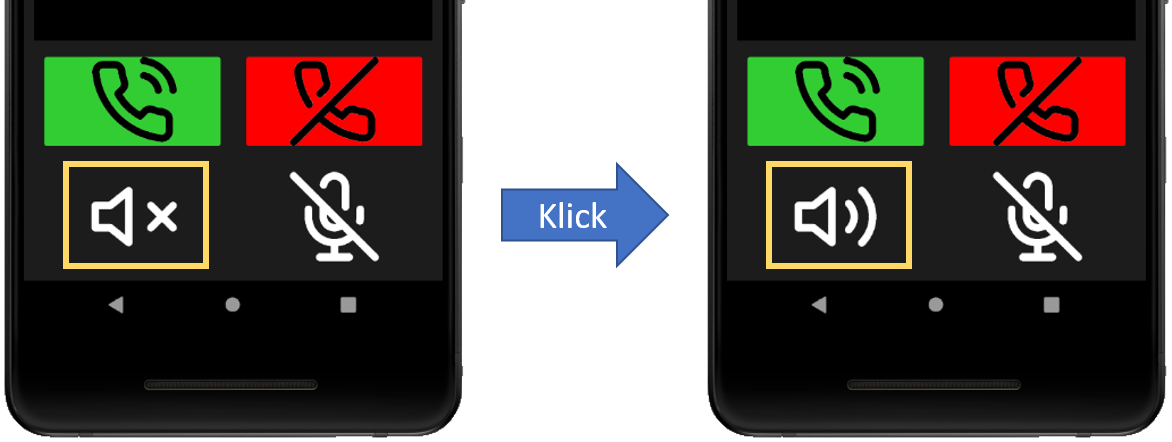
\includegraphics[width=.8\linewidth]{images/xamarin/VisualStateManager.png}
    \caption{VisualStateManager}
    \label{fig:visualstatemanager}
\end{figure}

Die hier beschriebenen Konzepte werden mehrmals verwendet, um die Oberfläche aufzubauen. Die Datei als Gesamtheit ergibt die in Bild \ref{fig:mainpage} gezeigte Oberfläche.
\begin{figure}
    \centering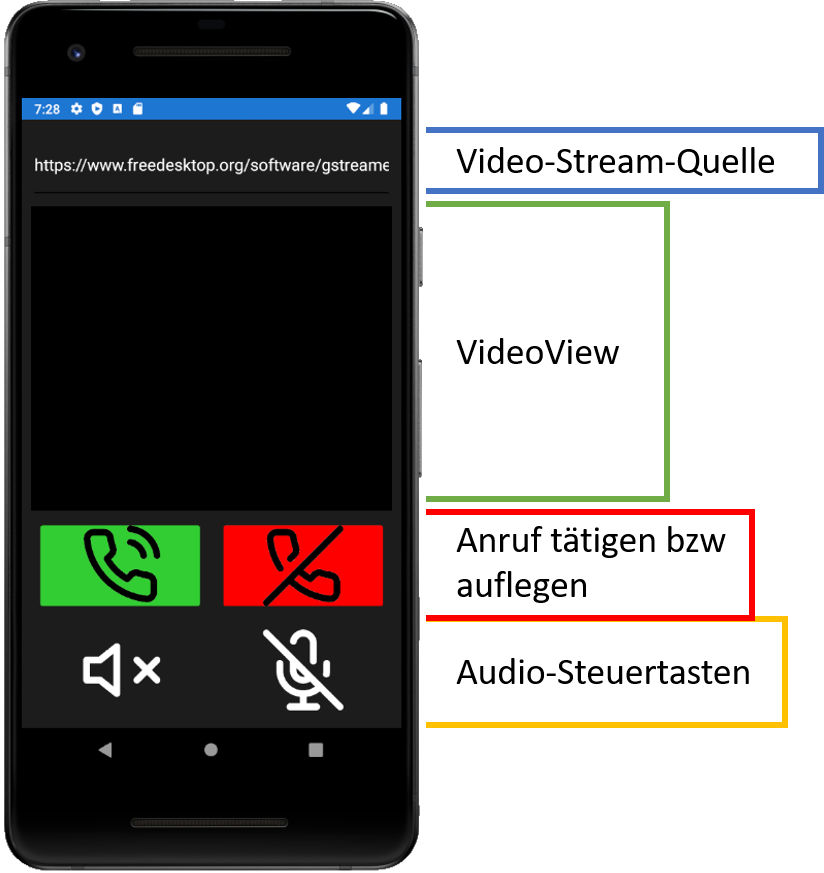
\includegraphics[width=.7\linewidth]{images/xamarin/MainPage.png}
    \caption{App-Oberfläche}
    \label{fig:mainpage}
\end{figure}

\subsection{MainPage.xaml.cs}
\label{ssec:mainpage-xaml-cs}
Dieser Teil beinhaltet den C\#-Code, der für die Steuerung und Verwaltung der Oberfläche notwendig ist.
Unter anderem wird hier das Verhalten beim Wechseln zwischen Hoch- und Querformat festgelegt.
\begin{minted}[firstnumber=36]{csharp}
    if (!AppCenter.Configured)
        Push.PushNotificationReceived += async (sender, e) =>
        {
#if DEBUG
            Console.WriteLine("DEBUG - Push-Notification recieved");
#endif
            foreach (string key in e.CustomData.Keys)
            {
#if DEBUG
                Console.WriteLine($"DEBUG - Custom Data: {key}:{e.CustomData[key]}");
#endif
                if (key == "mrl")
                    _player.Mrl = e.CustomData[key].ToString();
            }

            if (await DisplayAlert("Incoming Call", "Connect now?", "Yes", "No"))
            {
                _player.StartCall();
                _streamer.StartCall();
            }
        };
\end{minted}
Hier wird das Verhalten bei eingehender Push Benachrichtigung festgelegt.
\paragraph{39,41,44,46:} Die mit \enquote{\#} beginnenden Anweisungen sind sogenannte Preprocessor-Statements, mit denen dem Compiler spezielle Anweisungen gegeben werden können.
Hier soll der Programmteil, der sich zwischen \texttt{\#if DEBUG} und \texttt{\#endif} befindet, nur im DEBUG-Modus verarbeitet werden.
Wenn ein anderer Compiler-Modus ausgewählt ist, werden diese Teile ignoriert.
\paragraph{42-49:} Mit einer Schleife werden alle Zusatzdaten der Benachrichtigung überprüft.
Wenn der Datensatz \texttt{mrl} enthalten ist, wird dessen Wert in \texttt{\_player.Mrl} gespeichert.
Der Wert stellt die Server-Adresse dar, von der der Video-Stream abgerufen werden soll.
\paragraph{51-55:} Der Benutzer wird per Popup gefragt, ob der Anruf entgegengenommen werden soll (Abb. \ref{fig:inc-call}).
\begin{figure}
    \centering
    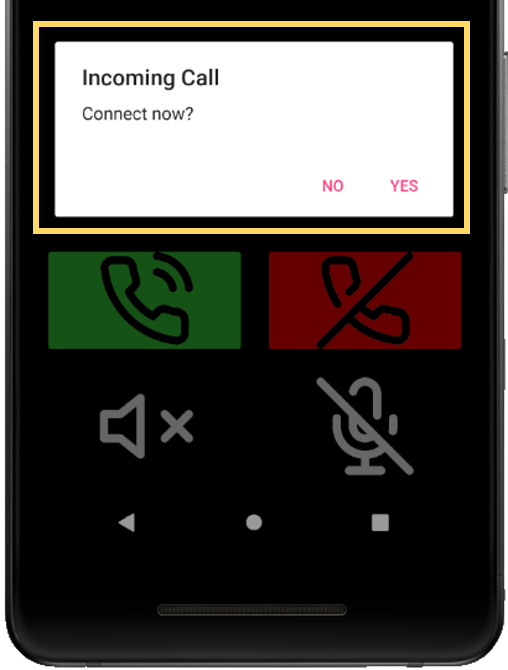
\includegraphics[width=.5\linewidth]{images/xamarin/IncomingCall.png}
    \caption{Abfrage Anrufannahme}
    \label{fig:inc-call}
\end{figure}
Wenn die Applikation in den Hintergrund geht, verliert die LibVLC die Referenz auf die VideoView und kann den Video-Stream nicht mehr darstellen.
Daher muss die Wiedergabe gestoppt werden, sobald die App in den Hintergrund geht, und neu gestartet werden, wenn die App wieder im Vordergrund ist.
Da die Benachrichtigung über den Vorder- bzw. Hintergrundstatus der Applikation nur über das native Projekt funktioniert, muss diese Information vom nativen Projekt zum portablen Projekt übertragen werden.
Dies geschieht mit der MessagingCenter-Komponente.
\begin{minted}[firstnumber=57]{csharp}
MessagingCenter.Subscribe<string>(this, "OnPause", app =>
{
    _wasConnected = _player.MediaPlayer.IsPlaying;
    _player.MediaPlayer.Pause();
    _prevPosition = _player.MediaPlayer.Position;
    _player.MediaPlayer.Stop();

    MainGrid.Children.Remove(VideoView);
});

MessagingCenter.Subscribe<string>(this, "OnRestart", app =>
{
    RegenerateVideoView();
    VideoView.MediaPlayer = _player.MediaPlayer;
    if (_wasConnected)
    {
        _player.MediaPlayer.Play();
        _player.MediaPlayer.Position = _prevPosition;
    }

    _prevPosition = 0;
});
\end{minted}
\paragraph{57-65:} Dieses Ereignis wird aufgerufen, wenn die Applikation in den Hintergrund wechselt.
Bevor dies geschieht, wird die aktuelle Wiedergabe-Position in einer Variablen gespeichert und die Wiedergabe gestoppt.
Anschließend wird die VideoView von der Oberfläche entfernt, damit sie später neu hinzugefügt werden kann.
\paragraph{67-78:} Das \texttt{OnRestart}-Event wird aufgerufen, wenn die App vom Hintergrund wieder in den Vordergrund geht.
Hier läuft derselbe Vorgang wie davor ab, jedoch in sinngemäß umgekehrter Reihenfolge.
Als erstes wird die VideoView der Oberfläche wieder hinzugefügt, damit die LibVLC eine Referenz dazu bilden kann.
Falls davor ein Video gespielt wurde, wird dieses fortgesetzt und die Variable für die vorherige Wiedergabeposition wird gelöscht.

\begin{minted}[firstnumber=84]{csharp}
BindingContext = _player;
\end{minted}
\paragraph{84:} Der BindingContext gibt für das \ac{mvvm}-Modell an, wo die Variablen, die mit der Oberfläche verknüpft sind, sich befinden.
In diesem Fall sind alle Variablen in der Player-Instanz \texttt{\_player} zu finden.

An folgender Funktion wird das Verhältnis von Oberflächenereignissen mit dem entsprechenden Code-Behind erklärt.
\begin{minted}[firstnumber=109]{csharp}
private void BtConnect_Clicked(object sender, EventArgs e)
{
    _player.StartCall();
    _streamer.StartCall("192.168.43.78");
}
\end{minted}
\paragraph{109:} Eine Funktion für ein Button-Event hat grundsätzlich als Rückgabe-Typ \texttt{void}, also nichts.
Auf die Funktion kann nur aus der selben Klasse zugegriffen werden, was mit dem \texttt{private}-Schlüsselwort bekanntgegeben wird.
Als Parameter werden Informationen zum Event-Auslöser und zum Event selbst mitgegeben.
\paragraph{111-112:} Wenn der grüne \enquote{Anrufen}-Button gedrückt wird, beginnen \texttt{\_player} und \texttt{\_streamer} damit, die Daten abzurufen bzw. bereitzustellen. Diese Funktionen werden im Abschnitt \ref{ssec:classes} genauer beschrieben.

Im letzten Abschnitt dieser Datei wird das Verhalten beim Wechseln zwischen Hoch- und Querformat festgelegt.
\begin{minted}[firstnumber=121]{csharp}
protected override void OnSizeAllocated(double width, double height)
{
    base.OnSizeAllocated(width, height);
    if (_width != width || _height != height)
    {
        _width = width;
        _height = height;
        if (width < height) //Portrait
        {
            MainGrid.ColumnDefinitions.Clear();
            MainGrid.ColumnDefinitions.Add(new ColumnDefinition
                {Width = new GridLength(1, GridUnitType.Star)});

            MainGrid.RowDefinitions.Clear();
            MainGrid.RowDefinitions.Add(new RowDefinition
                {Height = new GridLength(0.7, GridUnitType.Star)});
            MainGrid.RowDefinitions.Add(new RowDefinition
                {Height = new GridLength(3, GridUnitType.Star)});
            MainGrid.RowDefinitions.Add(new RowDefinition
                {Height = new GridLength(2, GridUnitType.Star)});

            Grid.SetColumnSpan(EditMrl, 1);
            Grid.SetColumn(ButtonGrid, 0);
            Grid.SetRow(ButtonGrid, 2);
        }
\end{minted}
[\dots]
\begin{minted}[firstnumber=164]{csharp}
    }
}
\end{minted}
\paragraph{121:} Die \texttt{OnSizeAllocated()}-Funktion ist eine vorgefertigte Funktion, die aufgerufen wird, wenn sich die Abmessungen der Oberfläche geändert haben.
Die neuen Abmessungen sind über die Parameter \texttt{width} und \texttt{height} verfügbar.
\paragraph{124-164:} Wenn die Abmessungen anders sind, als die Abmessungen beim letzten Aufruf wird das Oberflächen-Layout entsprechend angepasst.
Falls die Höhe länger als die Breite ist, greift der erste Teil der If-Else-Struktur, ansonsten der zweite.
\paragraph{130-144:} Zuerst werden die Reihen- und Spalten-Definitionen gelöscht, um sie neu zuweisen zu können.
Für das Hochformat werden eine Spalte und drei Reihen benötigt.
Diese werden mit den richtigen relativen Maßen hinzugefügt.
Wenn dies geschehen ist, werden die Oberflächenelemente den richtigen Plätzen im Grid zugewiesen.
\paragraph{146-163:} Das Verändern der Oberfläche für Querformat wird hier ausgelassen, da es sinngemäß äquivalent zum Hochformat ist.
\subsection{MediaClasses.cs}
\label{ssec:classes}
In dieser Source-Datei sind sämtliche Hilfsklassen zum Abrufen und Bereitstellen von Medieninformationen definiert.
Grundsätzlich finden sich hier zwei Klassen:
\begin{itemize}
    \item Player, die für das Abrufen des Medien-Streams vom Server und Darstellen von diesem zuständig ist
    \item Streamer, mit der das Zurückschicken der Mikrofon-Rohdaten erfolgen soll
\end{itemize}
\subsubsection{Player}
Die Player-Klasse implementiert das \ac{mvvm}-Modell, um die MediaPlayer-Komponente mit der Oberfläche zu verknüpfen.
Um die Anzeige über eine Änderung der Variablen zu informieren, muss der \texttt{PropertyChanged}-EventHandler mit dem Variablennamen als Argument aufgerufen werden.
Um die Lesbarkeit des Codes zu vereinfachen, wird dieser Aufruf meist in einem Unterprogramm versteckt, welches von Visual Studio automatisch generiert werden kann.
Daher wird auf den genauen Aufbau dieses Unterprogrammes nicht genauer eingegangen.
Die Initialisierung beinhaltet keine besonderen Funktionen und wird daher ebenfalls nicht behandelt.

\begin{minted}[firstnumber=36]{csharp}
public bool ToggleSpeaker()
{
    MediaPlayer.Volume = _speakerActive ? 0 : 100;
    return _speakerActive = !_speakerActive;
}
\end{minted}
\paragraph{38-39:} Über die Volume-Eigenschaft des MediaPlayer-Elements kann die Audio-Ausgabe in der Lautstärke verändert oder ganz abgeschaltet werden. Mit der Funktion \texttt{ToggleSpeaker()} wird der aktuelle Zustand der Ausgabe invertiert.
Das heißt, wenn die Ausgabe aktiviert ist, wird sie durch einen Aufruf des Unterprogrammes deaktiviert und umgekehrt.
Der neue Zustand wird als Wahrheitswert an die aufrufende Funktion zurückgegeben, wobei \texttt{true} bedeutet, dass die Audio-Ausgabe aktiv ist.
Als Abkürzung für ein mehrzeiliges If-Else-Statement wird der Ternary-Operator verwendet.
Diese Anweisung nimmt abhängig von einem Wahrheitswert zwei verschiedene Werte an.
Die Syntax dieser Abkürzung sieht so aus:
\begin{minted}{csharp}
variable = <true/false> ? <Wert wenn true> : <Wert wenn false>;
\end{minted}

Die \texttt{StartCall()}-Funktion wird aufgerufen, wenn der Benutzer auf den grünen Knopf drückt.
\begin{minted}[firstnumber=42]{csharp}
public void StartCall()
{
    MediaPlayer.Media = new Media(LibVlc, Mrl, FromType.FromLocation);
    MediaPlayer.Play();
    MediaPlayer.Volume = _speakerActive ? 100 : 0;
}
\end{minted}
\paragraph{44:} Bevor die MediaPlayer-Komponente ein Video abrufen kann, muss erst definiert werden, wo dieses Video zum Abruf bereitsteht. 
Über die Variable \texttt{Media} kann die Medieninformation des Ziel-Videos festgelegt werden. Die Variable \texttt{Mrl} stellt hier die aktuelle Adresse des Video-Streams dar.
\paragraph{45-46:} Mit der \texttt{Play()}-Funktion kann anschließend, wie der Name vermuten lässt, die Wiedergabe gestartet werden.
Jedoch wird im gleichen Zug die Wiedergabe-Lautstärke zurückgesetzt, weshalb sie nach dem Aufruf der \texttt{Play()}-Funktion wieder dem aktuell gewünschten Zustand der Audio-Wiedergabe angepasst werden muss.\par

\begin{minted}[firstnumber=49]{csharp}
public void EndCall()
{
    MediaPlayer.Stop();
}
\end{minted}
\paragraph{49:} Die Wiedergabe des Video-Streams kann am Ende des Gesprächs mit der \texttt{Stop()}-Funktion beendet werden.

Die C\#-Sprache bietet aufgrund der strengen Objektorientierung das Sprachkonstrukt \enquote{Property} an.
Eine Property kann mit einer gewöhnlichen Variable verglichen werden, allerdings bietet sie zusätzlich \texttt{get}- und \texttt{set}-Funktionen an.
Diese Zusatzfunktionen werden aufgerufen, wenn auf den Wert der Property zugegriffen bzw. dieser verändert wird.
Dies wird anhand eines Beispiels erläutert:
\begin{minted}[firstnumber=54]{csharp}
private string _mrl;
public string Mrl
{
    get => _mrl;
    set
    {
        _mrl = value;
        OnPropertyChanged();
    }
}
\end{minted}
\paragraph{54:} Eine Property mit benutzerdefinierten \texttt{get}- und \texttt{set}-Funktionen benötigt eine zusätzliche Variable, die den eigentlichen Wert der Property speichert.
Diese kann auch dann \texttt{private} und somit nach außen versteckt sein, wenn die Property selbst \texttt{public}, also von außen zugänglich ist.
\paragraph{57:} Die \texttt{get}-Funktion ist bei den meisten Properties so definiert, dass der Wert der internen Variablen einfach weitergegeben wird, da beim Auslesen in den meisten Fällen keine zusätzliche Aktion erforderlich ist.
\paragraph{58-62:} In der \texttt{set}-Funktion wird hier nicht nur der Wert der internen Variable mit dem neuen Wert überschrieben, sondern auch das System über eine Änderung informiert.
Dies ist für die Funktion des \ac{mvvm}-Modells essenziell.
\subsubsection{Streamer}
Die Streamer-Klasse ist deutlich kürzer, als die Player-Klasse, da die Streamer-Klasse selbst keine wirkliche Funktionalität beinhaltet.
Vielmehr dient diese Klasse als Interface zu den plattformspezifischen Softwaremodulen, die für die Audioaufnahme zuständig sind.
Dies wird mit Hilfe eines DependencyService erreicht.
\begin{minted}[firstnumber=90]{csharp}
private IAudioRecordingService Service { get; set; }

public Streamer()
{
    Service = DependencyService.Get<IAudioRecordingService>();
}
\end{minted}
\paragraph{94:} Der DependencyService dient als \enquote{Fernsteuerung}, mit dem vom portable Projekt ausgehend Ereignisse und Funktionen im nativen Code aufgerufen werden können.

\begin{minted}[firstnumber=112]{csharp}
public interface IAudioRecordingService
{
    void Start(IPEndPoint target);
    void Stop();
    bool ToggleMic();
}
\end{minted}
\paragraph{112-117:} Mit einem \texttt{interface} wird festgelegt, welche Funktionen eine Klasse, die von diesem abgeleitet wird, haben muss.
In diesem Fall muss der plattformspezifische Teil der Audioaufnahme die Funktionen \texttt{Start()}, \texttt{Stop()} und \texttt{ToggleMic()} definieren, um mit dem Interface kompatibel zu sein.
Über ein Interface können nicht nur Funktionen, sondern auch Variablen und Properties vorgegeben werden.


\section{PiBell.Android}
Dieses Projekt beinhaltet den gesamten nativen Code für die Android-Plattform.
Dazu gehören das Berechtigungs-Management, sowie die Audio-Aufnahme.

\subsection{MainActivity.cs}
Ähnlich wie bei Abschnitt \ref{ssec:app-xaml-cs} wird hier das native Android-Projekt initialisiert.
Dazu gehört das Laden aller Runtime-Ressourcen und des benötigten Programm-Codes, sowie Überprüfen bzw. Anfragen der Berechtigungen.
\begin{minted}[firstnumber=33]{csharp}
if (CheckSelfPermission(Manifest.Permission.RecordAudio) != Permission.Granted)
{
    RequestPermissions(new[] { Manifest.Permission.RecordAudio }, 1);
}
\end{minted}
\paragraph{33-36:} Es wird überprüft, ob die Berechtigung für die Audio-Aufnahme bereits erteilt ist.
Wenn das nicht der Fall ist, wird diese beim System angefragt.
Der Benutzer erhält dann ein PopUp, mit dem er gefragt wird, ob die Berechtigung erteilt werden soll.
Der Benutzer kann anschließend entweder, wie in Abbildung \ref{fig:permission} gezeigt, die Berechtigung erteilen oder verweigern.
In letzterem Fall kann die Applikation nicht richtig funktionieren.
\begin{figure}
    \centering
    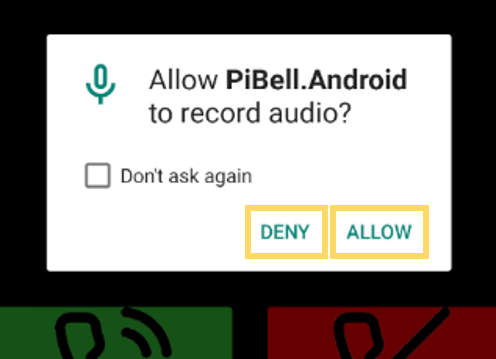
\includegraphics[width=.5\linewidth]{images/xamarin/permissionRequest.png}
    \caption{Anfrage für Berechtigung}
    \label{fig:permission}
\end{figure}

\begin{minted}[firstnumber=39]{csharp}
protected override void OnPause()
{
    base.OnPause();
    MessagingCenter.Send("app", "OnPause");
}

protected override void OnRestart()
{
    base.OnRestart();
    MessagingCenter.Send("app", "OnRestart");
}
\end{minted}
\paragraph{39-49:} Das in Abschnitt \ref{ssec:mainpage-xaml-cs} beschriebene Verhalten beim Wechsel der App von und in den Hintergrund benötigt ein vom nativen Projekt ausgelöstes Ereignis.
Über das MessagingCenter wird eine Nachricht an das portable Projekt geschickt, damit dieses den Zustandswechsel mitbekommt und darauf reagieren kann.
%\blindtext
%audio recording service
%permissions
%OnPause(), OnRestart()
